\chapter{Introducción}
\label{chap:introduccion}

\drop{E}{ste} primer capítulo pretende ofrecer una visión global de lo que el lector encontrará en este texto. El objetivo del presente es la construcción de un sistema informático completo, extensible y centrado en la mejora de diferentes habilidades mentales. No obstante, de ningún modo se centra exclusivamente en aspectos de la Ingeniería Informática, sino que ofrece un componente importante de estudio biológico centrado en comprender el funcionamiento del cerebro humano. Por supuesto, ese componente neurológico se plantea desde un punto de vista no experto en el tema, lo que facilita su comprensión por parte de personas ajenas al campo de la biología o la medicina.

Dado que, de cara al usuario final del sistema, BreakBrain es una red social, en primer lugar se realizará una introducción al aspecto social del Internet de hoy en día. Posteriormente se darán algunas pinceladas sobre el funcionamiento del cerebro humano, introduciendo conceptos elementales que más adelante serán desarrollados en profundidad. Por último, se ofrecerá una aproximación breve al entrenamiento cerebral mediante juegos.


\section{Redes sociales}

En la actualidad la mayoría de sitios web populares cuentan con un importante aspecto social. La compartición de contenido entre internautas es parte fundamental de su utilización, llegando incluso a tratarse del único propósito de algunos de estos sitios web.

Las redes sociales constituyen el máximo exponente de esa posibilidad de compartición, permitiendo mantener diferentes tipos de relaciones sociales entre los integrantes de las mismas. En la actualidad existen numerosas redes sociales, más o menos importantes. Las más conocidas y de mayor éxito son redes sociales dedicadas al ocio, en las que los usuarios comparten fotografías y comentarios, crean eventos, etc. No obstante, existen redes sociales de muy diversa índole en Internet, dedicadas al deporte, al cine, al desarrollo software, etc. No debemos ver esta abundancia como una sobresaturación de mercado, sino sencillamente entender que el aspecto social es la esencia de la web hoy en día.

\section{El cerebro humano}

El cerebro humano tiene una estructura similar al del resto de animales, pero destaca por su gran tamaño (en comparación con el resto del cuerpo). Este mayor tamaño proviene especialmente de lo que se conoce como {\it corteza cerebral}\index{córtex/corteza} ---o {\it córtex}---. El córtex es una cubierta que envuelve al cerebro, con una textura repleta de pliegues que posibilita que quepa en el cráneo.

La corteza cerebral se divide físicamente en dos hemisferios similares, que se encuentran, a su vez, divididos funcionalmente en cuatro lóbulos (figura \ref{fig::lobulos}):

\begin{figure}[h]
  \begin{center}
    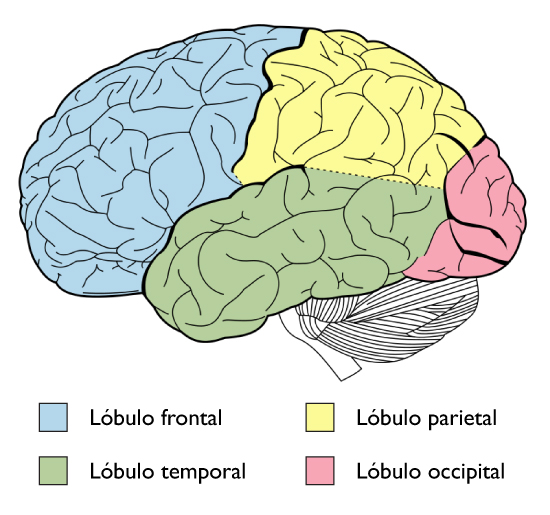
\includegraphics[scale=0.5]{images/lobulos.jpg}
    %http://www.wikisaber.es/uploadedImages/Recursos/Especial_Cuerpo_Humano/Lobulos_cerebrales.jpg
    \caption{Lóbulos cerebrales}
    \label{fig::lobulos}
  \end{center}
\end{figure}

\begin{itemize}
\item {\bf Lóbulo frontal}\\
Controla la capacidad de movimiento, razonamiento, resolución de problemas, lenguaje y emociones.
\item {\bf Lóbulo parietal}\\
Se encarga de las percepciones sensoriales externas (como manos y pies): sensibilidad, tacto, percepción, presión, temperatura y dolor.
\item {\bf Lóbulo temporal}\\
Se encarga de la audición, equilibrio y coordinación. Recibe y procesa información de los oídos y regula las emociones y motivaciones, como ansiedad, placer e ira.
\item {\bf Lóbulo occipital}\\
Se encarga del procesamiento de la visión y la producción de imágenes.
\end{itemize}

A lo largo de este texto se estudia la composición del cerebro humano en detalle, atendiendo tanto a aspectos arquitecturales como funcionales. Se ha realizado un análisis algo superficial ---sin entrar en detalles muy complejos---, con el único fin de servir como base al presente proyecto. Debe recordarse que el objetivo de este escrito es la elaboración de un sistema informático. No obstante, se han utilizado fuentes ampliamente reconocidas en el campo de la medicina.

El lector se verá sorprendido con pequeñas curiosidades históricas sobre las que se apoyan los conceptos explicados durante el análisis cerebral. El objetivo de las mismas no es otro que facilitar su lectura, ayudando a entender cómo se ha llegado a deducir el funcionamiento de cada área del cerebro.

\subsection{La neuroplasticidad}
\label{sec::neuroplasticidad}\index{neuroplasticidad}

El cerebro humano es un sistema dinámico de redes neuronales con gran potencial de evolución. La plasticidad cerebral, o {\it neuroplasticidad}, es precisamente esa capacidad dinámica que posee el cerebro, que le permite mejorar con el aprendizaje y repetición de ciertos ejercicios, y en la que se basa este proyecto. En la sección \ref{neuroplasticidad} se estudiará en profundidad este concepto, mencionando la evolución de su sensibilidad en base a la evolución del cuerpo humano y comentando algunos estudios interesantes sobre el tema.

Se relacionará la neuroplasticidad con el dolor y estrés crónicos, y se introducirá el interesante concepto del {\it cambio cualitativo}, comparándolo con el entrenamiento por repetición e introduciendo así la idea del entrenamiento cerebral mediante juegos.

\section{El entrenamiento cerebral mediante juegos}

Si hay algo que resulta realmente atractivo para el ser humano es la posibilidad de sobrepasar sus limitaciones, ya sea de forma física ---mediante el deporte--- o de forma mental ---mediante el entrenamiento cerebral---. En este sentido la utilización de pequeños juegos resulta una forma muy amena de hacerlo.

Existen diversos artículos dedicados, total o parcialmente, al estudio del entrenamiento cerebral mediante la práctica de juegos. Algunos artículos, como \cite{Hackley2011}, destacan el éxito de los juegos dedicados al entrenamiento cerebral, como el ``Dr. Kawashima's Brain Training'', de Nintendo. Otros utilizan la mejora obtenida mediante juegos como punto de partida para realizar otros estudios. Un buen ejemplo es \cite{Hirvasoja2004}, donde se estudia el efecto de la práctica de juegos sobre la percepción espacial de los seres humanos, comparando las mejoras obtenidas en función de la edad y el sexo.

La sección \ref{sec::fisiologia} se dedica al estudio del cerebro y desglose del conjunto de habilidades mentales estimulables. Más adelante, en la sección \ref{sec:entrenamiento} se especifica el entrenamiento de esas habilidades mediante los juegos de BreakBrain.

\section{Estructura del documento}

A continuación se ofrece una pequeña descripción del contenido de cada capítulo de este documento:

\begin{definitionlist}

\item [Capítulo \ref{chap:introduccion}: \nameref{chap:introduccion}] Este capítulo sirve como presentación del proyecto, explicando el contexto en el que se enmarca y dando unas primeras pinceladas sobre el desarrollo del mismo.

\item [Capítulo \ref{chap:objetivos}: \nameref{chap:objetivos}] En este capítulo se presentan las motivaciónes que desembocaron en el desarrollo de Breakbrain, así como los objetivos que persigue el mismo, tanto el objetivo general como los diferentes objetivos específicos en los que se desglosa.

\item [Capítulo \ref{chap:antecedentes}: \nameref{chap:antecedentes}] En este capítulo se presenta un análisis sobre el estado del arte en el que se enmarca el proyecto. Se analizarán las tecnologías y herramientas en las que se basa su desarrollo, así como algunos sistemas software precedentes que han servido de inspiración u ofrecen cierta semejanza con el proyecto que nos ocupa. Se presenta además, como pilar fundamental del desarrollo de BreakBrain, un estudio general sobre la anatomía y fisiología cerebral humana.

\item [Capítulo \ref{chap:metodo}: \nameref{chap:metodo}] En este capítulo se explica la metodología seguida durante el desarrollo del sistema informático que supone este proyecto. Se hará un recorrido detallado por todas las etapas del mismo, desde el primer estudio de requisitos hasta la realización de pruebas de diferentes tipos, presentando cada artefacto generado durante el proceso.

\item [Capítulo \ref{chap:arquitectura}: \nameref{chap:arquitectura}] En este capítulo se ofrece una visión detallada de la composición de BreakBrain. Se hará especial hincapié en el despliegue del sistema, los patrones utilizados y la extensibilidad de la plataforma.

\item [Capítulo \ref{chap:resultados}: \nameref{chap:resultados}] En este capítulo se ofrecerá una especificación precisa sobre el entrenamiento cerebral mediante juegos ---para cada una de las áreas mencionadas--- diseñado para BreakBrain.

\item [Capítulo \ref{chap:conclusiones}: \nameref{chap:conclusiones}] En este capítulo se realiza una valoración de los objetivos alcanzados, así como propuestas de futuro y una opinión personal sobre el desarrollo del proyecto.

\item [Anexo \ref{chap::iteraciones}: \nameref{chap::iteraciones}] Este anexo contiene el desglose iterativo del desarrollo de BreakBrain, obtenido a partir de la aplicación del Proceso Unificado de Desarrollo.

\item [Anexo \ref{chap::instalacion}: \nameref{chap::instalacion}] Este anexo muestra el proceso necesario para instalar y ejecutar BreakBrain.

\item [Anexo \ref{chap::guia}: \nameref{chap::guia}] Este anexo ofrece una guía detallada para el desarrollo de juegos para la plataforma.

\item [Anexo \ref{chap::manual}: \nameref{chap::manual}] Este anexo ofrece un manual de usuario para aprender a manejar BreakBrain de una forma sencilla.

\end{definitionlist}

